\chapter{Software}
\begin{figure}[htb]
  \centering  
  
\includegraphics[scale=0.5]{img/soft/logo.png}
  \caption{Software Logo}
  \label{sec:logo}
\end{figure}

\label{sec:software}
\section{Anforderungen und Programmaufbau}
\subsection{Kurze Beschreibung}
\begin{itemize}
\item Auftraggeber und Auftragnehmer vereinbaren ein Werkstoffprüfungsprojekt.
Das Prüfverfahren besteht aus verschiedenen Methoden, eine heißt Radiation-Test,
die Durchstrahlungsprüfung, ein bildgebendes Verfahren der
zerstörungsfreien Werkstoffprüfung (ZFP) zur Darstellung von Materialunterschieden.
Mit Röntgen- oder Gammastrahlung aus einer geeigneten Quelle (einer Röntgenröhre,
einem Elektronenbeschleuniger mit Röntgentarget oder
einem gammastrahlenden Radionuklid) wird die Dichte eines Bauteils auf
einem Röntgenfilm abgebildet.
Dort erscheint ein Projektionsbild des Bauteils. Am Grad der Schwärzung lässt sich die
unterschiedliche Materialdicke oder -dichte erkennen. Je dicker oder dichter ein Bauteil,
desto weniger Strahlung kann es durchdringen und desto heller erscheint die Stelle auf dem
Röntgenbild.
\item Der Auftragnehmer bildet ein Arbeitsteam für das Projekt.
\item Das Arbeitsteam besteht wie folgt aus:
\begin{enumerate}
\item Personal - Radiograph, mindestens zwei Personen
\item Materialien
\item Personal - Teamleiter, der gleichzeitig auch Radiograph sein kann
\item Personal health physics Safety (HPS) als Schnittstelle zwischen \\Atomenergie-Behörde, Radiographen und Auftragnehmer zur Koordinierung der Sicherheitsverfahren.
\end{enumerate}
\item Programmaufbau:
\begin{itemize}
\item Model
\begin{itemize}
\item Project
\begin{enumerate}
\item Team
\begin{enumerate}
\item Materialien (Siehe \ref{sec:resourcen})
\item Personal HPS,Radiographer und Assistance
\begin{enumerate}
\item Sicherheit (Siehe \ref{chap:Sicherheit})
\end{enumerate}
\end{enumerate}
\end{enumerate}
\end{itemize}
\item Server (Teil \ref{sec:server})
\begin{itemize}
\item PlayFramework version 2.5.15 mit Java und Scala.
\item Datenkommunikation mit dem WebSocket-Protokoll.
\end{itemize}
\item Android-Client (Teil \ref{sec:client})
\begin{itemize}
\item USER: Health Physics Safety(HPS)\\
(Bild: \ref{sec:hps})
\item USER: Radiographer\\
(Bild: \ref{sec:rg})
\end{itemize}
\end{itemize}
\end{itemize}

\section{Anforderungen und die Spezifikation}
\begin{enumerate}
\item Jedes Projekt kann aus einer Werkstoffprüfung (RT) oder mehreren Werkstoffprüfungen
(RT+MT) bestehen.\\
\subsubsection{in Server package models;}

\begin{lstlisting}[frame=single]

public enum TYPE {RT, PT, MT, UT, LT,VT;
    @Override
    public String toString() {
        return "TYPE{}" + super.toString();
    }
    
 public class Team {
 private TYPE type;
 
 public Team(List<Personal> personals,TYPE type) {
        this.personals = personals;
        this.setType(type);
        this.setTeamReport("TEAM START REPORT");
        this.setLocation(LOCATION.CENTRAL);
        switch (getType()) {
            case RT:
                if (personals.size() < 2) {
                    log.inf(("Number of persons is less than 2"));
                    setStatus(false);
                }
                break;
            case MT:
                //TODO
                break;
            case ET:
                //TODO
                break;
            case LT:
                //TODO
                break;
            case PT:
                //TODO
                break;
            case UT:
                //TODO
                break;
            case VT:
                //TODO
                break;

        }

        this.id = DATA.creatId("-" + getType().name().toString());
        this.setName(getId() + "_TEAM");
        instanceCounter++;
        counter = instanceCounter;
    }
   } 

\end{lstlisting}

\item Die Durchstrahlungsprüfung kann mit einem Elektronenbeschleuniger mit Röntgentarget
X-Ray oder einem gammastrahlenden Radionuklid durchgeführt werden.
\begin{lstlisting}[frame=single]
public enum ISOTOPETYPE {
    IRIDIUM_192, SELENIUM_75, COBALT_60, YTTERBIUM_169, CAESIUM_137, X_Ray100KV, X_Ray200KV, X_Ray220KV, X_Ray120KV, LINAC_8MeV,OTHER;
    @Override
    public String toString() {
        return "ISOTOPETYPE{} " + super.toString();
    }
}
\end{lstlisting}
\item Jedes Prüfungsverfahren in einem Projekt sollte alle nötigen Materialien zur Verfügung
haben.\\
\begin{lstlisting}[frame=single]
public class MATERIAL {
    private String name;
    private String model;
    private TYPE type;
    private String SerialNumber;
    private ServerLog log = new ServerLog();
    private boolean isStatus;
    public MATERIAL(String name, TYPE type) {
        setName(name);
        setModel(DATA.creatId("-" + name));
        setSerialNumber(DATA.generateUniqueId());
        setType(type);
        log.info("NEW OBJECT CREATED,NAME:  " +getClass() + "");


    }
  }
\end{lstlisting}
\item Die Strahlung des Bunkers muss gemessen werden und im System eingegeben werden.\\
\begin{lstlisting}[frame=single]
public class SafetyActivity extends Activity {
 private List<Item> items;
 
 @Override
    protected void onCreate(Bundle savedInstanceState) {
     super.onCreate(savedInstanceState);
        setContentView(R.layout.activity_items);
     items = new ArrayList<>();
     items.add(new Item("Inside bunker  INFO max 7.5  muSv/h"));
     items.add(new Item("Outside bunker INFO max 2.5  muSv/h"));
    }
}
\end{lstlisting}
\item Aktuelle Position (Standort) der RT-Kamera sollte der/ dem Verantwortlichen für HPS
mitgeteilt werden.\\
\begin{lstlisting}[frame=single]
public enum LOCATION {
    CENTRAL, PROJECT, ATOMENERGIE_INSTITUT, ONTHEWAY;
       @Override
       public String toString() {
       return "LOCATION{} " + super.toString();
    }
}
\end{lstlisting}
\item Grenze der Gammastrahlung des RT-Bunkers, wo die RT-Kamera gelagert wird, muss nach
dem Standard berechnet werden.\\
\begin{lstlisting}[frame=single]
public class SafetyActivity extends Activity {
 private List<Item> items;
 
 @Override
    protected void onCreate(Bundle savedInstanceState) {
     super.onCreate(savedInstanceState);
        setContentView(R.layout.activity_items);
    items = new ArrayList<>();
    items.add(new Item("On camera max 2 mSv/h"));
    items.add(new Item("1m distance from camera max 20 muSv/h"));
    }
}
\end{lstlisting}

\item Falls die Sicherheitsmaßnahmen verletzt wurden, sollte sofort die/der HPS-Verantwortliche
informiert werden und zusätzliche Sicherheitsmaterialien gelistet sein.\\
\begin{lstlisting}[frame=single]
public class AlarmActivity extends Activity {

 @Override
    protected void onCreate(Bundle savedInstanceState) {
    super.onCreate(savedInstanceState);
        setContentView(R.layout.activity_items);
        //Create model list
        items = new ArrayList<>();
        final String EMERGENCY_MESSAGE =
                "1 : Remote Handling tongs " + "\n" +
                "2: Shielded container" + "\n" +
                "3: Hand tools -> wrench,pliers,croppers" + "\n" +
                "4: Fist aid kit" + "\n" +
                "5: Radiation warning labels & signs" + "\n" +
                "6: Barriers/ropes" + "\n" +
                "7: call HPS";
                
                
        items.add(new Item("ALARM", "RADIATION EMERGENCY MESSAGE", EMERGENCY_MESSAGE));
        items.add(new Item("ALARM", "RADIATION EMERGENCY MESSAGE"));
        //send Alarm Message to HPS 
 client.getWebSocket().send(ToJson.sendObjectWithRoot("ALARM FROM",personal).toString()); 
    }
}
\end{lstlisting}
\item Die Warnungsmaßnahmen werden automatisch aktiv, indem die/der HPS-Verantwortliche
Warnungsnachrichten erhält.\\
\begin{lstlisting}[frame=single]
    //send Alarm Message to HPS 
 client.getWebSocket().send(ToJson.sendObjectWithRoot("ALARM FROM",personal).toString());
\end{lstlisting}
\item Nach Beendigung der Warnungsmaßnahme wird der/die HPS-Verantwortliche detailliert
über die Hintergründe und Ursachen der Verletzung der Sicherheit in Kenntnis gesetzt.
\begin{lstlisting}[frame=single]
    //Report  
 public class ReportActivity extends AppCompatActivity implements DatePickerDialog.OnDateSetListener, View.OnClickListener {
 }
\end{lstlisting}
\item Desweiteren erhält der/die HPS-Verantwortliche die aktuellen Daten zur Strahlenbelastung
nach dem Ende der Warnungsmaßnahme.\\
\begin{lstlisting}[frame=single]
    //Report  
 public class ReportActivity extends AppCompatActivity implementsDatePickerDialog.OnDateSetListener, View.OnClickListener {
 }
\end{lstlisting}
\item Anhand der Eigenschaft der RT-Kamera sowie deren maximalen Kapazität sollte das richtige
Isotop darauf geladen werden; bei falschem Isotop sollte die RT-Kamera nicht aktiviert und
die/der HPS-Verantwortliche informiert werden.\\
\begin{lstlisting}[frame=single]
  public class RT_Camera extends Observable {
  private ArrayList<ISOTOPETYPE> isotopetypes;
  
   /**
     * @param model of RT Camera and here will be check capacity safety!
     */
    private void setDevice_Source_Maximum_Capacity(MODEL model, Isotope isotope) {
        switch (model) {
            case SIGMA_880:
                this.isotopetypes.add(ISOTOPETYPE.SELENIUM_75);
                this.isotopetypes.add(ISOTOPETYPE.IRIDIUM_192);
                this.isotopetypes.add(ISOTOPETYPE.COBALT_60);
                this.isotopetypes.add(ISOTOPETYPE.YTTERBIUM_169);
                this.isotopetypes.add(ISOTOPETYPE.CAESIUM_137);
                if (isotope.getIsotopetype().equals(ISOTOPETYPE.SELENIUM_75) && isotope.getActivity() <= 150) {
                    this.setCapacityPermision(true);
                    this.setIsotopes(isotope);
                }
                //130Ci 4.81TBq
                if (isotope.getIsotopetype().equals(ISOTOPETYPE.IRIDIUM_192) && isotope.getActivity() <= 130) {
                    this.setCapacityPermision(true);
                    this.setIsotopes(isotope);
                }
                // 0.025 Ci = 25mCi
                if (isotope.getIsotopetype().equals(ISOTOPETYPE.COBALT_60) && isotope.getActivity() <= 0.025) {
                    this.setCapacityPermision(true);
                    this.setIsotopes(isotope);
                }

                if (isotope.getIsotopetype().equals(ISOTOPETYPE.YTTERBIUM_169) && isotope.getActivity() <= 20) {
                    this.setCapacityPermision(true);
                    this.setIsotopes(isotope);
                }

                //0.38 Ci = 380mCi
                if (isotope.getIsotopetype().equals(ISOTOPETYPE.CAESIUM_137) && isotope.getActivity() <= 0.38) {
                    this.setCapacityPermision(true);
                    this.setIsotopes(isotope);
                }
                break;
                case OMEGA_880:
                .........
      }
  
  }
\end{lstlisting}
\item Eine passive RT-Kamera darf nicht für ein Projekt zur Verfügung stehen.\\
\begin{lstlisting}[frame=single]
public class RT_Camera extends Observable {
 private boolean capacityPermision;
 private boolean isotopeTypePermision;
}
\end{lstlisting}

\item Das Projekt muss mit allen jeweiligen Voraussetzungen vorbereitet werden, sodass man
täglich genaue Informationen über das Projekt erhält und alle Projekte mit zugehörigen
Teilen bekannt bleiben bis das Projekt beendet ist.
\begin{lstlisting}[frame=single]
//-------Project------
public class Project {
 private List<Team> teams = new LinkedList<>();
 //---------
 for(Team t:teams){
 	t.getTeamReport();
 }
}
//------- Team--------
public class Team {
 private String teamReport;
}

\end{lstlisting}
\item In das System sollten die Sicherheitsmaßnahmen sowie Sicherheitsdistanzen für Mitarbeiter
eingegeben und dokumentiert werden.Area1,Area2 und Area3.
\begin{lstlisting}[frame=single]
public class SafetyActivity extends Activity {
 private List<Item> items;
 
 @Override
    protected void onCreate(Bundle savedInstanceState) {
     super.onCreate(savedInstanceState);
        setContentView(R.layout.activity_items);
    items = new ArrayList<>();
   //-------Area----------
  items.add(new Item("forbidden_area Forbidden area (Aktivity >= 2 mSv/h)"));
  items.add(new Item("control_area Control area(2 mmuSv/h >Aktivity>25 muSv/h)"));
  items.add(new Item("free_area Free area (25 muSv/h > Aktivity)"));

    }
    //--------Safety Warning Message-------
      if (isWarning) {
    client.getWebSocket().send(ToJson.message(
    "Safety Warning", personal.getId(),warning).toString());
     isWarning = false;
     setReceiveMessage(client.getReceiveMessage());
                            
   }
}
\end{lstlisting}
\item Das Prüfobjekt sollte als Parameter im System eingegeben werden.
\begin{lstlisting}[frame=single]
public class TimeActivity extends Activity implements View.OnClickListener {
 private void updateThickness() {
   if (getThickness() < 5) {
            setThickness(5);
            text_view_Ft_warning.setText("Thickness=5");
            Toast.makeText(TimeActivity.this, getResources().getString(R.string.value_is_false, text_view_Ft_warning.getText()), Toast.LENGTH_LONG).show();
            text_view_Ft_warning.setText("5mm<= t >=74mm");
        }
    }
}


//-------------TestObject Array---------------
<string name="material">MATERIAL</string>
    <string name="material_prompt">Choose a Material</string>
    <string-array name="material_arrays">
        <item>Iron</item>
        <item>Steel</item>
        <item>Lead</item>
        .....
        .....
        .....
    </string-array>
\end{lstlisting}

\item Das Programm sollte für die Verbesserung des Tests die Zeit des Gammastrahlen-Shootings
und die Distanz des Isotops \grqq Strahlungsquelle\grqq zum Prüfobjekt berechnen.
\begin{lstlisting}[frame=single]
public class TimeActivity extends Activity implements View.OnClickListener {

    //----------radiation Time-------------------
    /**
     * @param ff  Film Factor
     * @param t   Thickness
     * @param sfd Distance of Film from Source
     * @param A   Source Activity
     * @return real radiation time
     */
    public double radiationTime(double ff, double t, double sfd, double A) {
        double res = 0;
        t = metal_Thickness_Factor((int) t);
        res = ff * t * Math.pow(sfd, 2) / A * Math.pow(100, 2);
        realTime = res;
        return res;
    }
  
}

\end{lstlisting}
\item Falls das Prüfobjekt Rohrrundnähte hat, wird auch die Distanz zum Film berechnet.
\begin{lstlisting}[frame=single]
public class TimeActivity extends Activity implements View.OnClickListener {

 //----------radiation Real Time-------------------
  /**
     * @param film_factor
     * @param half_value_layer
     * @param distance_film_from_source
     * @param gamma_Factor_RHM
     * @param sourceActivity
     * @return realTime
     */
    public double radiationRealTime(double film_factor, int half_value_layer, double distance_film_from_source, double gamma_Factor_RHM, double sourceActivity) {
        double res = 0;
        res = ((film_factor * Math.pow(2, 1 / half_value_layer) * Math.pow(distance_film_from_source, 2) * 60) / (gamma_Factor_RHM * sourceActivity * Math.pow(100, 2)));
        time = res;
        return res;
    }
 }
\end{lstlisting}

\item Das Programm sollte so realisiert werden, dass die Kommunikation zwischen
Zentralniederlassung, HPS und Radiograph erleichtert wird.\\
\subsubsection{Kommunikation zwischen Radiographer and HPS}
\begin{itemize}
\item Server: (\ref{sec:server})
\item Client: (\ref{sec:client})
\begin{itemize}
\item  Android-Client Health Physics Safety (HPS)
\item  Android-Client Radiograp
\end{itemize}
\end{itemize} 
\item Der/Die HPS sollte die aktuellen Informationen über den Radiographen 
nach Auswertung von dessen TLD und Film Badge Dosimeter im System dokumentieren.
\begin{lstlisting}[frame=single]
public class Personal {
    private TLD tld;
    private FilmBadge filmBadge;
    private GeigerAlarm geiger;
    private PocketDosimeter dosimeter;
}
public abstract class DOSIMETER {
    private String serialNumber;
    private boolean calibration;
    private String calibrationDate;
    private String calibrationExpire;
    private LOCATION location;
    private boolean status;
    private String calibrationMessage;
    private String value;
}
public class TLD extends DOSIMETER {}
public class FilmBadge extends DOSIMETER {}
public class Radiometer extends DOSIMETER {}
public class PocketDosimeter extends DOSIMETER {}
\end{lstlisting}
\item Die Kalibration eines Messgerätes sollte nicht abgelaufen sein.
\begin{lstlisting}[frame=single]
public abstract class DOSIMETER {
    private boolean calibration;
    private String calibrationMessage;
     /**
     * check calibration expert
     * @return boolean
     */
    public boolean isCalibration() {
        boolean result = getCalibrationExpire() == DATA.getDate();
        if (result) {
            this.setCalibrationMessage("CALIBRATION EXPERT");
        }
        return calibration;
    }
}
\end{lstlisting}
\item Zwei Wochen vor Ablaufdatum der Kalibration sollte der/die HPS-Verantwortliche informiert
werden, an welchem Standort sich das Gerät befindet.
\begin{lstlisting}[frame=single]
public abstract class DOSIMETER {
    private boolean calibration;
    private String calibrationMessage;
    /**
     * send message to HPS for Calibration
     * in two weeks, the calibration will expire
     */
    public void calibrationMessage() {

        if (getCalibrationExpire() == DATA.addNewDayToDate(-14)) {
            this.setCalibrationMessage("IN TWO WEEKS, THE CALIBRATION WILL BE EXPIRED.");
        }
    }
 }
\end{lstlisting}
\item Teammitglieder arbeiten nach dem Rotationsprinzip. Das bedeutet, nach einer aktiven Phase
geht einer der Mitarbeiter in eine passive Phase, dafür übernimmt ein anderer Mitarbeiter
den aktiven Part bis zum nächsten Wechsel.
\item Ein Team besteht aus mindestens zwei Personen, die durch spezielle Schulungen zertifiziert worden sind.
\item Im Team kann auch eine weitere Person als Assistent fungieren, die nicht unbedingt geschult worden ist. Jedoch muss diese Person mit allen Sicherheitsmaßnahmen und entsprechenden
Materialien zum Schutz vertraut sein.
\end{enumerate}

\subsection{SBT-Server}
\label{sec:server}
Server besteht aus den folgenden Teilen:
\begin{itemize}
\item PlayFramework version  2.5.15 mit Java und Scala.\\
\textcolor{blue}{\textbf{\textup{https://www.playframework.com}}}
\item Datenkommunikation mit dem WebSocket-Protokoll:\\
%% URL
\textcolor{blue}{\textbf{\textup{https://tools.ietf.org/html/rfc6455}}}
\subsubsection{Datenkommunikation}

Das WebSocket-Protokoll ist ein auf TCP basierendes Netzwerkprotokoll, das entworfen wurde, um eine bidirektionale Verbindung zwischen einer Webanwendung und einem WebSocket-Server bzw. einem Webserver, der auch WebSockets unterstützt, herzustellen.
\subsubsection{Inhaltsverzeichnis}
\begin{enumerate}
\item Vorteile gegenüber reinem HTTP:\\
Während bei einer reinen HTTP-Verbindung jede Aktion des Servers eine vorhergehende Anfrage des Clients erfordert, reicht es beim WebSocket-Protokoll, wenn der Client die Verbindung öffnet. Der Server kann dann diese offene Verbindung aktiv verwenden und kann neue Informationen an den Client ausliefern, ohne auf eine neue Verbindung des Clients zu warten.

Eine vom Server initiierte Übertragung ist bei einer reinen HTTP-Verbindung nur durch verzögertes Antworten auf eine vom Client initiierte Anfrage möglich (long polling).

Zudem entfallen bei WebSockets die durch den HTTP-Header verursachten zusätzlichen Daten, die bei jeder Anfrage einige Hundert Bytes umfassen können.

Technisch betrachtet startet bei WebSocket, wie bei HTTP, der Client eine Anfrage, mit dem Unterschied, dass nach der Übertragung der Daten zum Verbindungsaufbau die zugrundeliegende TCP-Verbindung bestehen bleibt und Übertragungen in beide Richtungen ermöglicht.


\item Der WebSocket-Protokoll-Handshake:\\
Zu Beginn jeder Verbindung führen Server und Client einen sogenannten Handshake durch. Dieser ähnelt dem HTTP-Header und ist vollständig abwärtskompatibel zu diesem, was die Nutzung des Standard-HTTP-Ports „80“ zugleich für normale HTTP-Kommunikation als auch für die Websocket-Nutzung ermöglicht. Der Handshake beinhaltet außerdem weitere Informationen (z. B. die verwendete Protokollversion).
\begin{enumerate}
\item Anfrage des Clients:\\
Die Anfragen landen in Class Interface.java,\\deren Methode \textcolor{red}{\textbf{OnRecive(Object message)}}.\\



\begin{lstlisting}[frame=single]
  
    @Override
    public void onReceive(Object message) {
        if (message instanceof String) {
            this.setJsonFactory(this.getMapper().getFactory());
            JsonFactory factory = mapper.getFactory();
            try {
                System.out.println(" Receive Message in OnReceive Server : " + message);
                parser = factory.createParser((String) message);
                this.setParser(jsonFactory.createParser((String) message));
                this.setJsonNode(this.getMapper().readTree(this.getParser()));
                if (this.getJsonNode() != null) {
                    this.messageActor(this.getJsonNode());
                } else {
                    this.getLog().info("You have null jsonNode");
                }
            } catch (IOException e) {
                e.printStackTrace();
            }

        } else {
           
            System.out.println("Type of your jsonNode is not valid or not Json");

        }


    }
\end{lstlisting}

Hier werden die Nachrichten mit JsonKey in der Methode:\\ \textcolor{red}{\textbf{messageActor(JsonNode json)}} weiter orientiert.\\
\begin{lstlisting}[frame=single]


package actors.serverInterface;

public class Interface extends UntypedActor {
     * jsonNode Actors management for messages 
     *from Client and answer back to client
     * @param json
     */
    private synchronized void messageActor(JsonNode json)
     throws JsonProcessingException {

        String jsonKey = json.fields().next().getKey();
        
        
        //------------------Message Type ----------------
        
        
        switch (jsonKey) {
            case "Hello":
                this.out.tell(TOJSON.replayMessage("Hey Client , im Server ")
                .toString() + "\n", self());
                this.output(TOJSON.replayMessage("Hey Client , im Server"));
            break;
            case "Start":
                this.out.tell(TOJSON.message("Start", "OK")
                .toString() + "\n", self());
                this.output(TOJSON.message("Start", "OK"));
            break;
            
            
            case "PERSONAL":
                this.personal = Json.fromJson(json.get("PERSONAL"), Personal.class);
                lobby.addPersonalInLobby
                (this.personal);
             break;
             
             }
           }
          }  
\end{lstlisting}



\item Antwort des Servers:\\
Die Anfragen werden in \textcolor{red}{\textbf{Interface.Props}} \\
\begin{lstlisting}[frame=single]
	
    public static Props props(ActorRef out, Lobby lobby) {
        return Props.create((Class<?>) Interface.class, out, lobby);
    }
\end{lstlisting}

und in \textcolor{red}{\textbf{app.controllers.SocketController}}\\
\begin{lstlisting}[frame=single]

package controllers;

public class SocketController extends Controller {
    Lobby lobby=new Lobby();

    public LegacyWebSocket<String> getSocket() {
        return WebSocket.withActor
        (out -> Interface.props(out, lobby));
    }

}
\end{lstlisting}

 landen.
 Hier werden die Nachrichten mit der Methode:\\ \textcolor{red}{\textbf{LegacyWebSocket<String> getSocket()}} zum Client gesendet.\\
\textcolor{blue}{\textbf{Hinweis:}} routes path : GET  /getsocket  controllers.SocketController.getSocket()
\end{enumerate}
\end{enumerate}
\item Nachrichtenaustausch mit Jackson:\\
In Java verwendet Play die Jackson JSON-Bibliothek, um Objekte in und aus JSON zu konvertieren. Die Aktionen von Play arbeitet mit dem JsonNode-Typ und das Framework stellt Hilfsmethoden für die Konvertierung in der play.libs.Json-API bereit. 
\end{itemize}

\subsection{Android-Client}
\label{sec:client}
\begin{itemize}
\item Datenkommunikation mit dem WebSocket-Protokoll und Json/Gson Nachrichten.\\
\begin{itemize}
\item WebSocket für die Kommunikation mit Server.\\
\href{https://medium.com/@ssaurel/learn-to-use-websockets-on-android-with-okhttp-ba5f00aea988}{\color{blue}{Beispiel: Websocket on Android}}
\item Json: Externe Inhalte in Nachrichten.\\
\href{https://www.tutorialspoint.com/android/android_json_parser.htm}{\color{blue}{Beispiel: Json on Android}}
\item Gson: Interne Inhalte in Nachrichten.\\
\href{https://guides.codepath.com/android/leveraging-the-gson-library}{\color{blue}{Beispiel: Gson on Android}} 
\end{itemize}

\subsubsection{Datenkommunikation}

\begin{lstlisting}[frame=single]
/**
     * Structure of the Client and WebSocketListener */
     

package com.androidjson.firebasegooglelogin_androidjsoncom.connection;
   /**
     * Structure of Clinet */
public class Client {
private EchoWebSocketListener listener;
private static WebSocket webSocket;
private OkHttpClient client;

public Client() {
        this.setOkHttpClient(new OkHttpClient());
        setWebSocketListener(new EchoWebSocketListener(this));
        start();
        gson = new Gson();
    }
  /**
     * Structure of the Websocket
     *
     * 1) Request 
     *    1.1) 192.168.178.50 is SBT-Server IP
     *    1.2) 9000 SBT-Server Port
     *    1.3) getsocket is in SBT-Server fix
     *    
     * 2) OkHttpClient
     * 
     * 3) WebSocketListener
     * 
     * 4) WebSocket(okHttpClient.newWebSocket(request, webSocketListener))
     */
    public void start() {
        request = new Request.Builder().url("ws://192.168.178.50:9000/getsocket").build();
        if (request != null && webSocketListener != null) {
            setWebSocket(okHttpClient.newWebSocket(request, webSocketListener));
        } else {
            log.e(TAG, "Maybe server is not running");
            okHttpClient.dispatcher().executorService().shutdown();
        }

    }
    
     
    /**
     * @return websocket for send Message to Server
     */
    public synchronized static WebSocket getWebSocket() {
        return webSocket;
    } 
  
 } 
  
  
  
  
  /**
     * Structure of WebSocketListener */
     
 final class EchoWebSocketListener extends WebSocketListener {
  
  private Client c;

    public EchoWebSocketListener(Client c) {
        this.c = c;
    }
     @Override
    public void onOpen(WebSocket webSocket, Response response) {
        webSocket.send(ToJson.helloServer().toString() + "\n");
    }
    //------------Incoming Message--------------------- 
    @Override
    public void onMessage(WebSocket webSocket, String message) {
    
        if (message instanceof String) {
            this.messageConvector(message);
        }
    }

    @Override
    public void onClosing(WebSocket webSocket, int code,
    String reason) {
        webSocket.close(NORMAL_CLOSURE_STATUS, null);
        webSocket.close(NORMAL_CLOSURE_STATUS, "Goodbye !");
    }
    public void setReplayMsg(String replayMsg) {
        this.setReplayMsg(replayMsg);
    }
    
    
    
    
    
    
    
    
    
    
    //-------------- convert Receive Message------------
    private void messageConvector(String message) {
        ObjectMapper mapper = new ObjectMapper();
        JsonFactory factory = mapper.getJsonFactory();
        JsonParser jp = null;
        try {
            jp = factory.createJsonParser(message);
            JsonNode jsonNode = mapper.readTree(jp);
            messageActor(jsonNode);
        } catch (IOException e) {
            e.printStackTrace();
      }
    }
    
  
    
    
    
    
    
    
    
    
  
  
 
  
    //---------------------Receive Json Message-------------
    private synchronized void messageActor(JsonNode json) throws IOException {

        ObjectMapper mapper = new ObjectMapper();
        String jsonKey = json.fields().next().getKey();
        //------------------Message Type --------------
        switch (jsonKey) {
        case "Replay message":
             c.getWebSocket().send(ToJson.message("Start","I want to start")
             .toString() +"\n");
        break;
        case "Start":
            c.getWebSocket().send(ToJson.message("Client", "Thanks")
            .toString() + "\n");  
            c.getWebSocket().send(ToJson.message("PERSONALSLIST",
            "I NEED PERSONAL LIST").toString() +"\n");
        break;
           }
       }
  }
 
\end{lstlisting}
\item Authentifizieren mit Google-Anmeldung auf Android mit Firebase.\\
\begin{lstlisting}[frame=single]
public class MainActivity extends AppCompatActivity implements DatePickerDialog.OnDateSetListener,View.OnClickListener,  GoogleApiClient.ConnectionCallbacks,GoogleApiClient.OnConnectionFailedListener {
    private ImageView user_pic,
	 // Firebase Auth Object.
    public FirebaseAuth firebaseAuth;
    private FirebaseAuth.AuthStateListener mAuthListener;
    // Google API Client object.
    public GoogleApiClient googleApiClient;
    // Sing out and next buttons
    private Button signOut_btn;
    // Google Sign In button .
    private com.google.android.gms.common.SignInButton signInButton;
    @Override
    protected void onCreate(Bundle savedInstanceState) {
    	super.onCreate(savedInstanceState);
        setContentView(R.layout.activity_main);
        // Getting Firebase Auth Instance into firebaseAuth object.
        firebaseAuth = FirebaseAuth.getInstance();
        // Creating and Configuring Google Sign In object.
GoogleSignInOptions googleSignInOptions = new GoogleSignInOptions.Builder(GoogleSignInOptions.DEFAULT_SIGN_IN)
                .requestIdToken(getString(R.string.default_web_client_id))
                .requestEmail()
                .requestScopes(new Scope("profile"))
                .build();
                
        / Creating and Configuring Google Api Client.
        googleApiClient = new GoogleApiClient.Builder(MainActivity.this)
        .enableAutoManage(MainActivity.this, new GoogleApiClient.OnConnectionFailedListener() {
        @Override
        public void onConnectionFailed(@NonNull ConnectionResult connectionResult) {
              }
          } /* OnConnectionFailedListener */)
                .addApi(Auth.GOOGLE_SIGN_IN_API, googleSignInOptions)
                .build();
    }
     @Override
    protected void onActivityResult(int requestCode, int resultCode, Intent data) {

        super.onActivityResult(requestCode, resultCode, data);

        if (requestCode == RequestSignInCode) {

            GoogleSignInResult googleSignInResult = Auth.GoogleSignInApi.getSignInResultFromIntent(data);

            if (googleSignInResult.isSuccess()) {

                GoogleSignInAccount googleSignInAccount = googleSignInResult.getSignInAccount();

                FirebaseUserAuth(googleSignInAccount);


            }

        }

    }
    //--------------
        public void FirebaseUserAuth(GoogleSignInAccount googleSignInAccount) {
        AuthCredential authCredential = GoogleAuthProvider.getCredential(googleSignInAccount.getIdToken(), null);
        Toast.makeText(MainActivity.this, "login with: "+ authCredential.getProvider(), Toast.LENGTH_LONG).show();
        firebaseAuth.signInWithCredential(authCredential)
        .addOnCompleteListener(MainActivity.this, new OnCompleteListener<AuthResult>() {
                    @Override
                    public void onComplete(@NonNull Task<AuthResult> AuthResultTask) {
                        if (AuthResultTask.isSuccessful()) {
                            // Getting Current Login user details.
                            FirebaseUser firebaseUser = firebaseAuth.getCurrentUser();
                            String email = firebaseUser.getEmail().toString();
                            setEmail(email);
                            String name = firebaseUser.getDisplayName();
                            setFirstName(parsingName(name)[0].toString());
                            setLastName(parsingName(name)[1].toUpperCase());
                            pic= firebaseUser.getPhotoUrl().toString();
                            uri=firebaseUser.getPhotoUrl();
                            Picasso.with(getApplicationContext()).load(pic).into(user_pic);
         client.getWebSocket().send(ToJson.message("USER_EMAIL", email).toString()+ "\n");

                            userChecker(client);
                            // Showing Log out button.
                            signOut_btn.setVisibility(View.VISIBLE);
                            // Hiding Login in button.
                            signInButton.setVisibility(View.GONE);
                            // Showing the TextView.
                            LoginUserEmail.setVisibility(View.VISIBLE);
                            LoginUserName.setVisibility(View.VISIBLE);

                            // Setting up name into TextView.
LoginUserName.setText("Name:" + firebaseUser.getDisplayName().toString());
                            // Setting up Email into TextView.
LoginUserEmail.setText("E-Mail:" + firebaseUser.getEmail().toString());
                           

Toast.makeText(MainActivity.this, " Welcome "+ getFirstName() + "" + getLastName()+" to NDT Software ", Toast.LENGTH_SHORT).show();
                        } else {
        Toast.makeText(MainActivity.this, "Something Went Wrong", Toast.LENGTH_LONG).show();
                        }
                }
          });

    }
 }
\end{lstlisting}
\href{https://firebase.google.com/docs/auth/android/google-signin}{\color{blue}{Tutorial: Authenticate with Firebase}}\\
\href{https://www.androidhive.info/2016/06/android-getting-started-firebase-simple-login-registration-auth/}{\color{blue}{Beispiel: Login and Registration Authentication}}

\item  Android-Client Health Physics Safety (HPS)
\begin{itemize}
\item HPS verwendet ein Google-Benutzerkonto, um sich bei dem System anzumelden.\\
(Bild: \ref{sec:hps}) 
\item Projekt-Auswahl: 
\begin{itemize}
\item Eine Liste von Projekten
\end{itemize}
\item Teams-Auswahl:
\begin{itemize}
\item Eine Liste von Teams.
\item Mit dem letzten Item kann der User ein neues Team erzeugen.\\
Dafür müssen erst zwei Personen ausgewählt werden, damit die Material-Activity erscheint.\\
Hier können die Materialen für das Team erzeugt werden.
Danach kann User mit dem letzten Item das Team erzeugen. 
\end{itemize}
\item Personal-Auswahl:
\begin{itemize}
\item Eine Liste von Personen, die sich einmal im System registriert haben.
\end{itemize}
\item Messages-Auswahl:
\begin{itemize}
\item Eine Liste von Nachrichten, die von Radiographen gesendet worden sind.
\end{itemize}
\item Material-Auswahl:
\begin{itemize}
\item Eine Liste von Materialien, die User erzeugen kann.
\end{itemize}
\item Alarm-Auswahl:
\begin{itemize}
\item Hier kann HPS die Alarm-Funktion für Haupt-HPS einschalten.
\end{itemize}
\end{itemize}
\item  Android-Client Radiographer
\begin{itemize}
\item Radiographer verwendet ein Google-Benutzerkonto, um sich bei dem System anzumelden.\\
( Bild: \ref{sec:rg})
\item Safety-Auswahl:
\begin{itemize}
\item Eine Liste von den Sicherheitsmaßnahmen, die dokumentiert werden müssen. 

\end{itemize}
\item Report-Auswahl:
\begin{itemize}
\item Hier kann der Radiographer die verwendeten Filme dokumentieren und zum HPS senden.

\end{itemize}
\item Time-Auswahl:
\begin{itemize}
\item Für die Verbesserung des Tests wird die Zeit des Gammastrahlen-Shootings
      und die Distanz des Isotops \grqq Strahlungsquelle\grqq zum Prüfobjekt berechnet.
\end{itemize}
\item Material-Auswahl:
\begin{itemize}
\item Der Radiographer kann die nötigen Materialien nochmal anfordern. 
\end{itemize}
\item Alarm-Auswahl:
\begin{itemize}
\item Hier kann der Radiographer den HPS alarmieren.
\end{itemize}
\end{itemize}
\end{itemize}
%==================Android Bilder============================
\chapter{Android Bilder}
\section{Android Bilder}
\begin{figure}[htb]  
  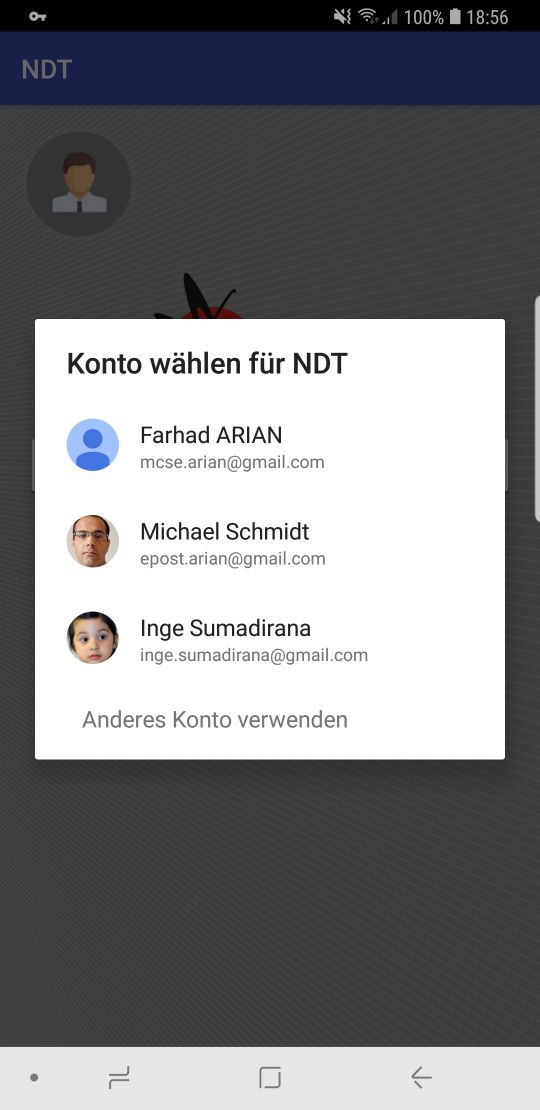
\includegraphics[scale=0.2]{img/soft/login.jpeg}
   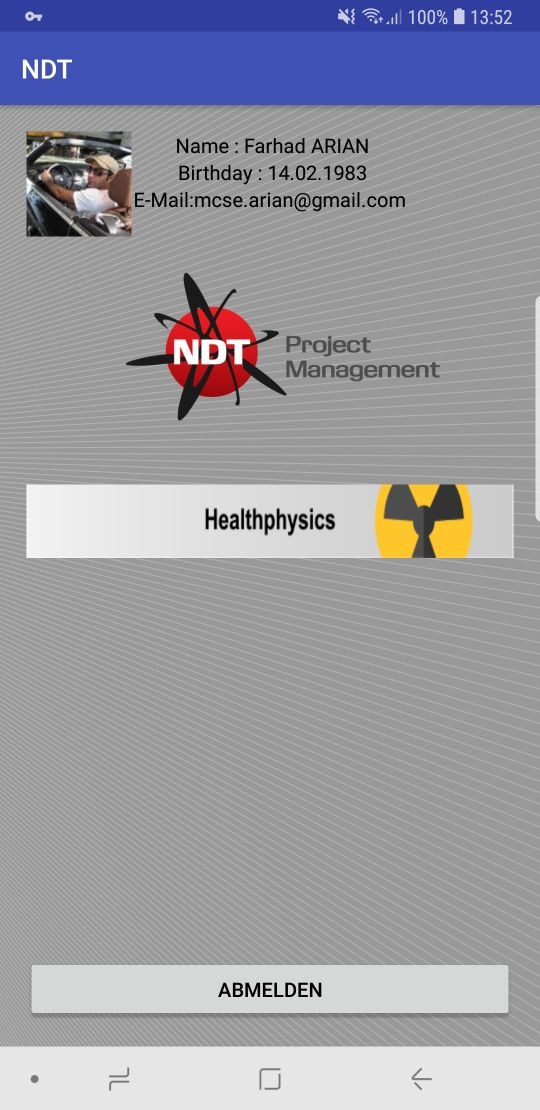
\includegraphics[scale=0.2]{img/soft/hps.jpeg}
    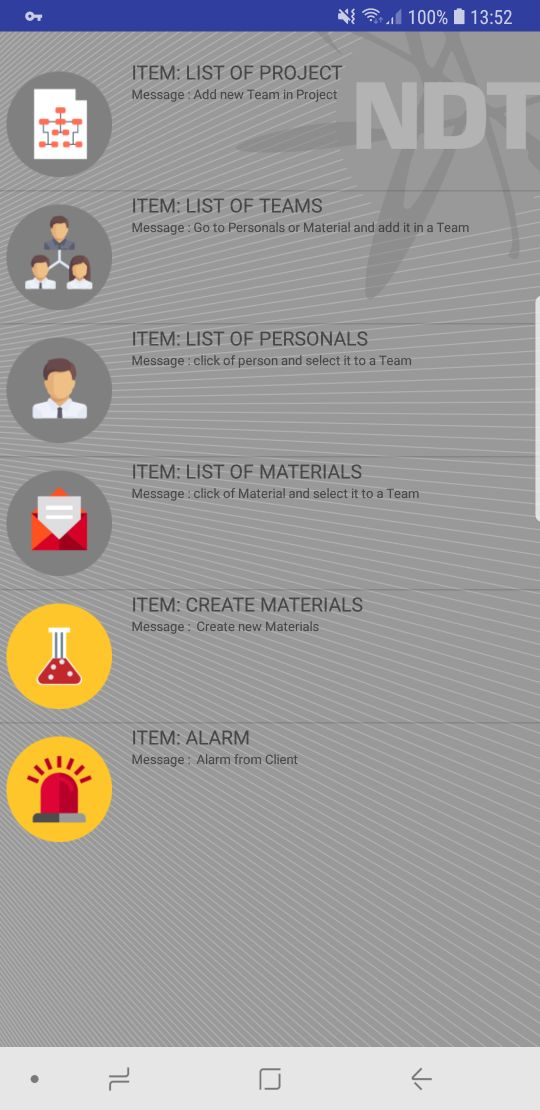
\includegraphics[scale=0.2]{img/soft/hps_start.jpeg}
     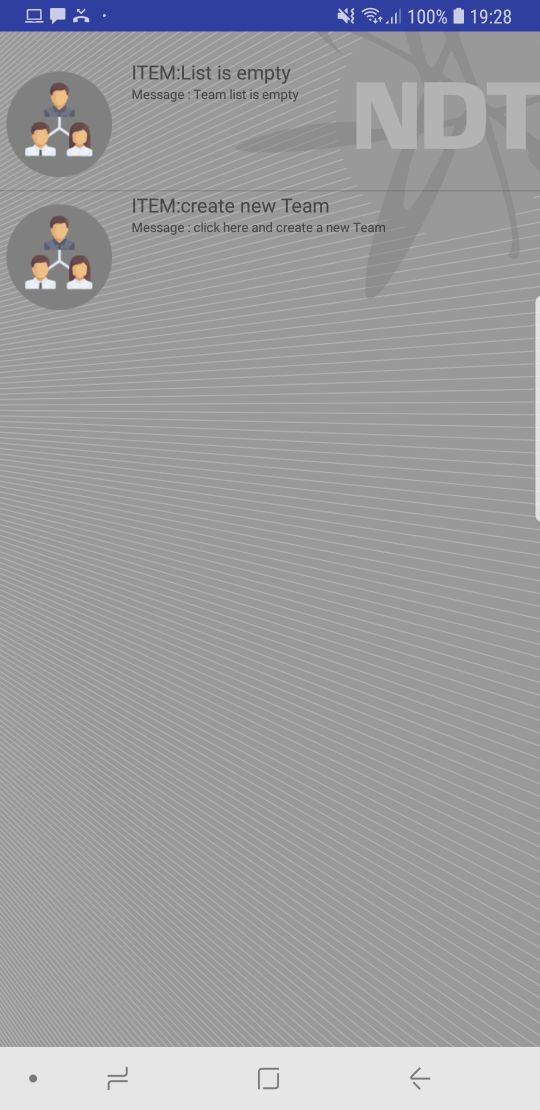
\includegraphics[scale=0.2]{img/soft/teamistEmpty.jpeg}\\
      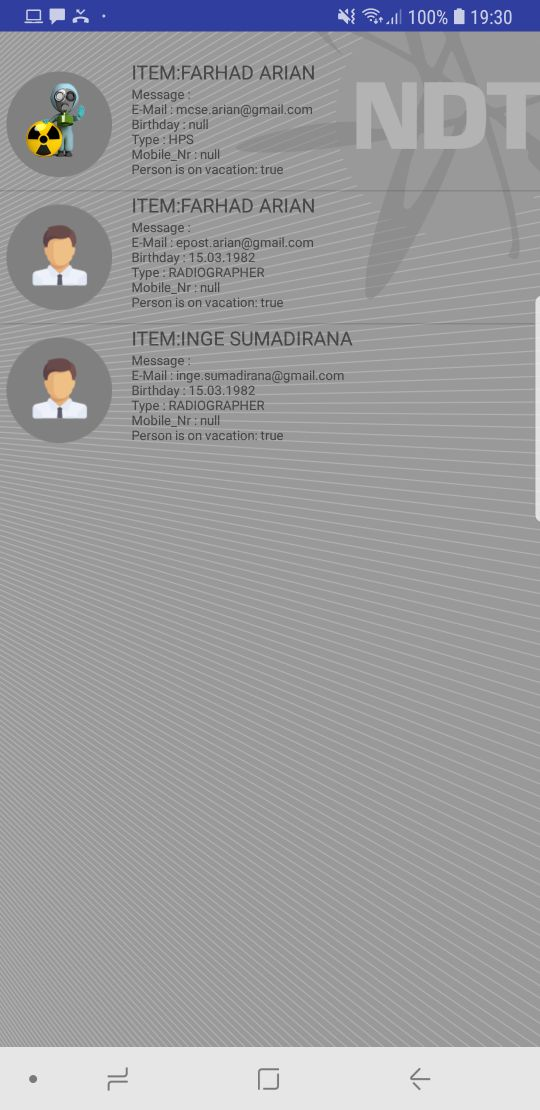
\includegraphics[scale=0.2]{img/soft/listOfPersonals.jpeg}
       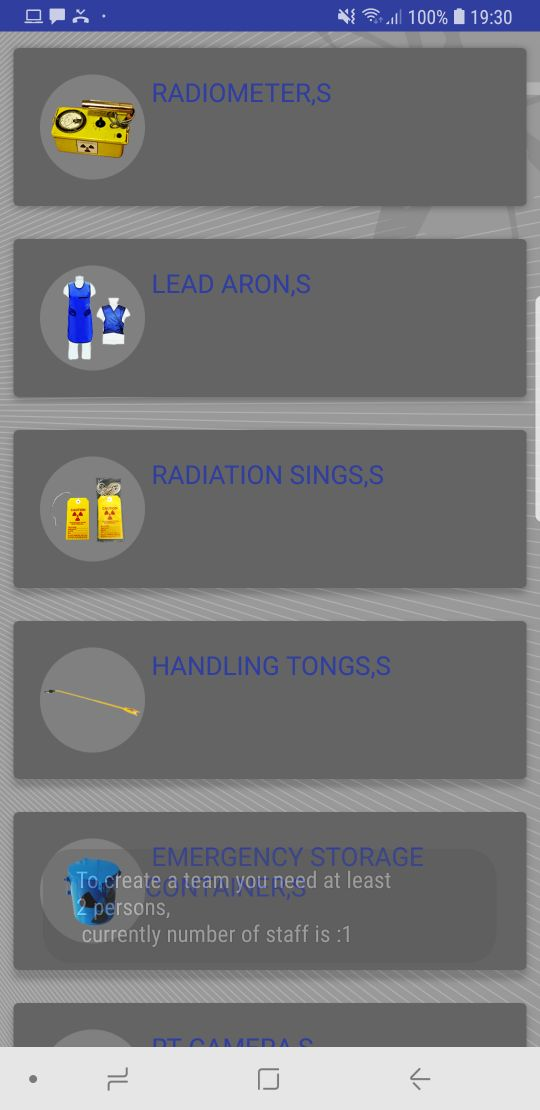
\includegraphics[scale=0.2]{img/soft/materialcreateforTeam.jpeg}
        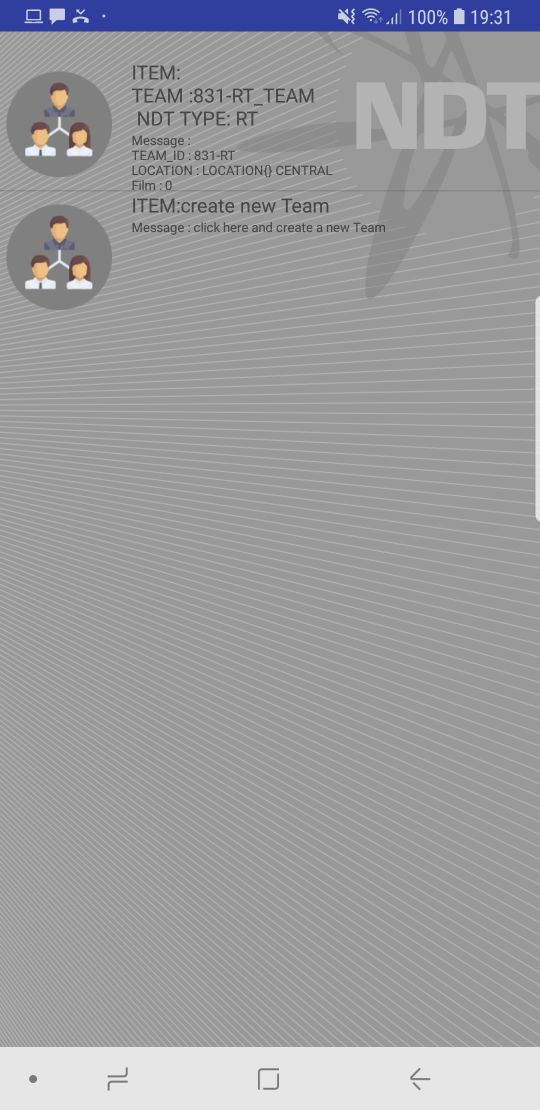
\includegraphics[scale=0.2]{img/soft/newTeam.jpeg}
         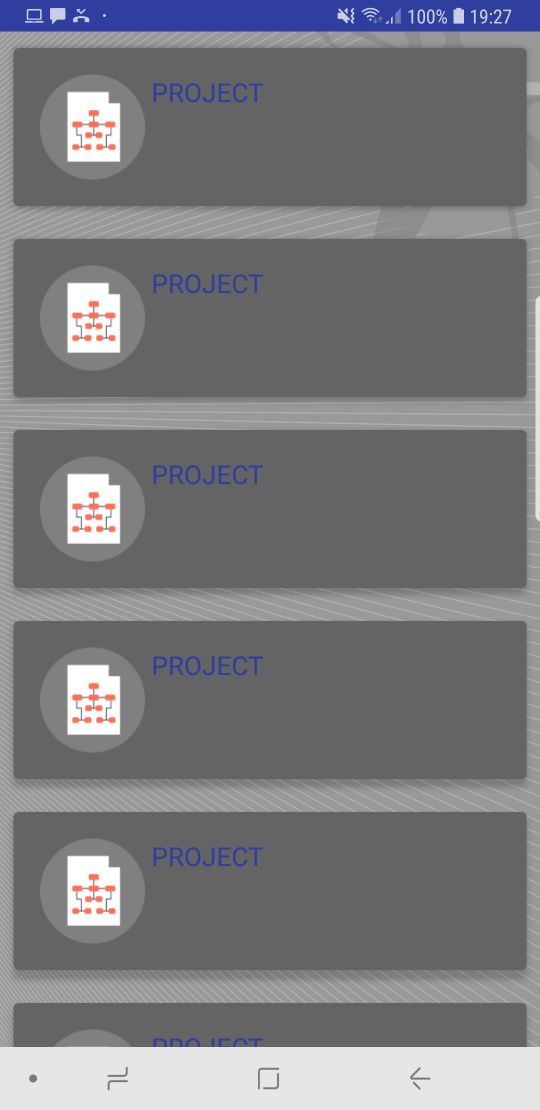
\includegraphics[scale=0.2]{img/soft/project.jpeg}\\
  \caption{Android-Client HPS}
  \label{sec:hps}
\end{figure}
\begin{figure}[htb]
   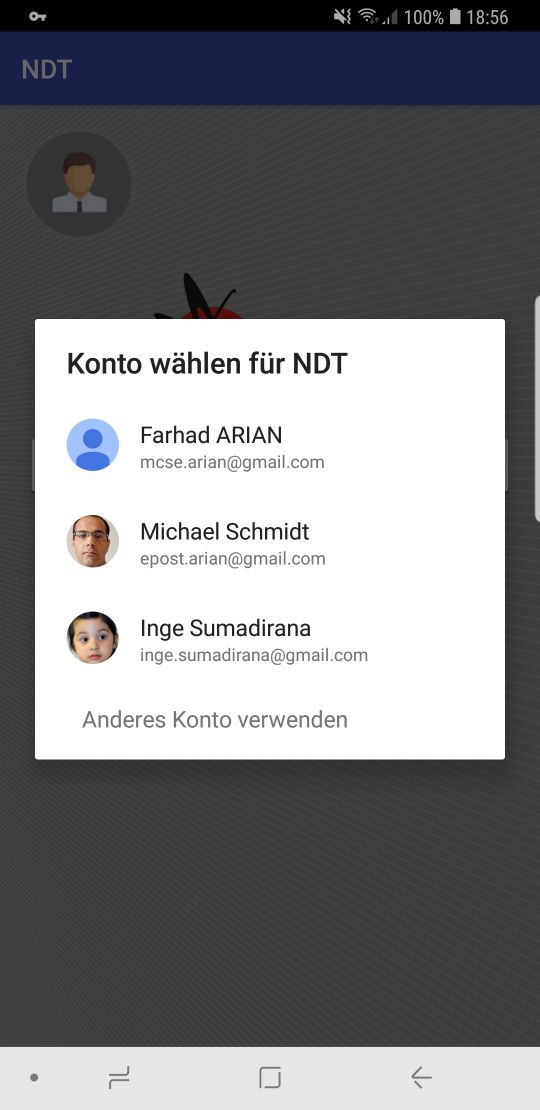
\includegraphics[scale=0.2]{img/soft/login.jpeg}
   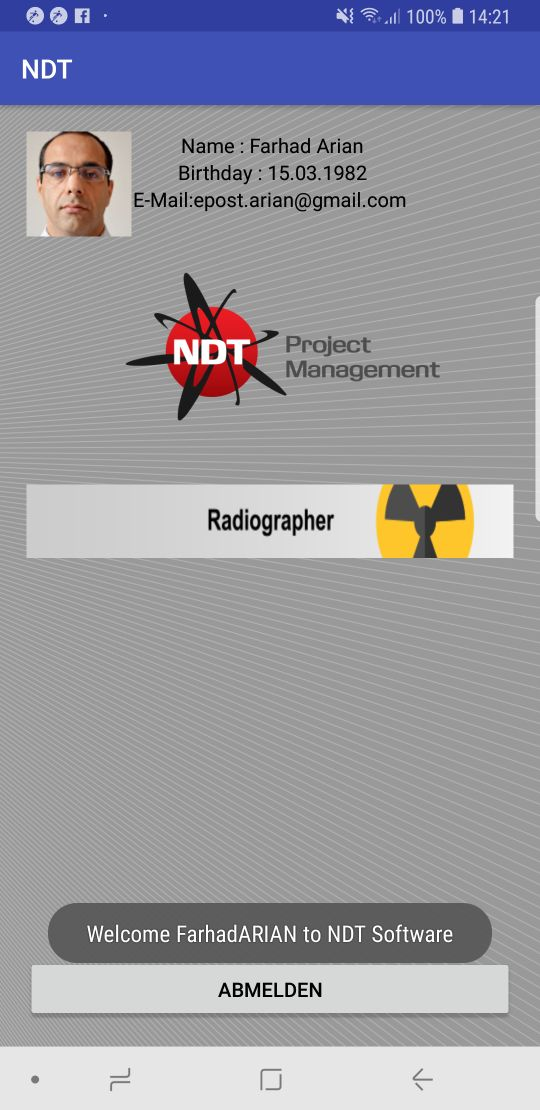
\includegraphics[scale=0.2]{img/soft/radiographer.jpeg}
    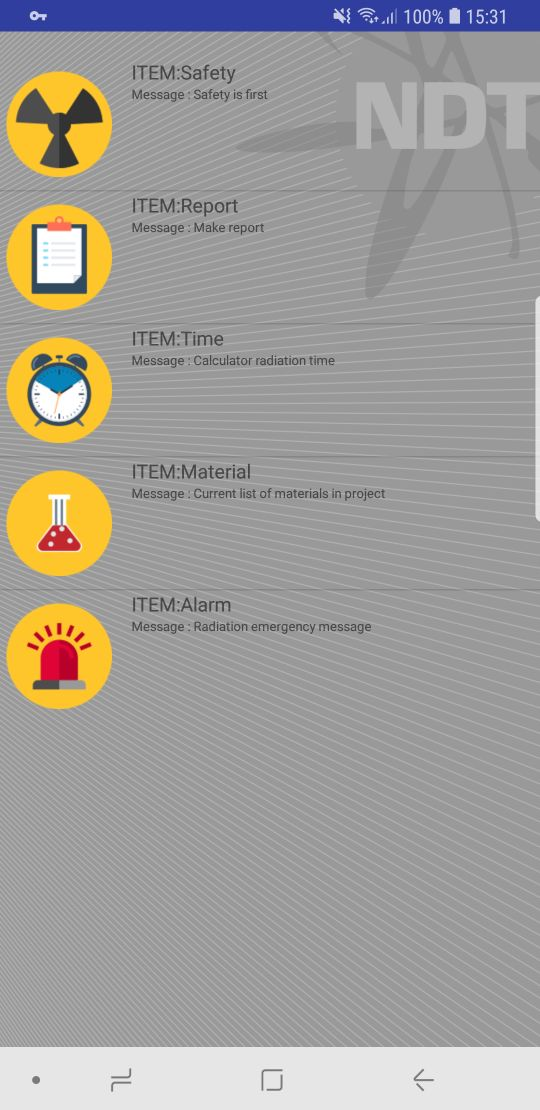
\includegraphics[scale=0.2]{img/soft/rg_start.jpeg}
     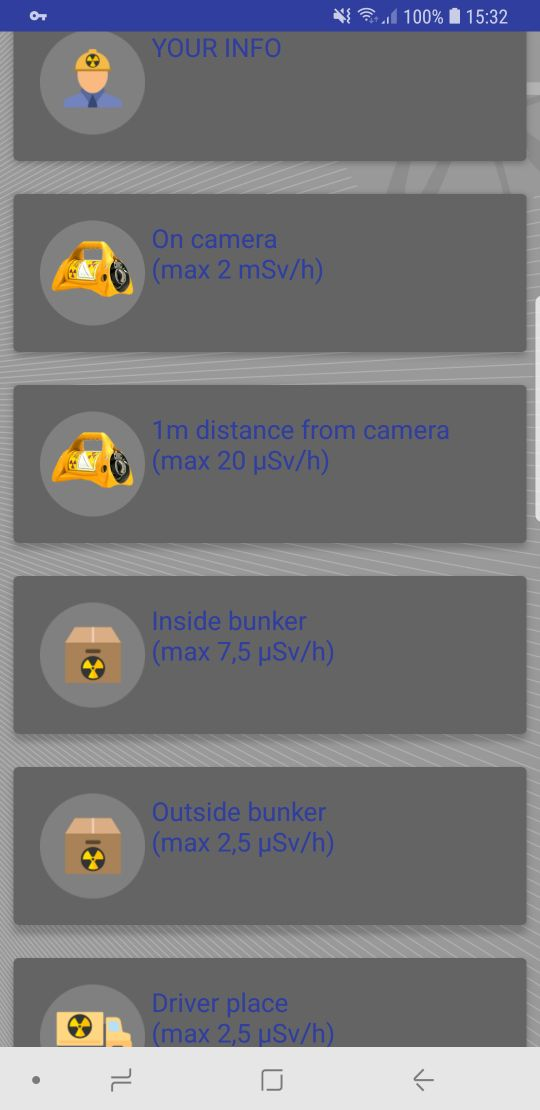
\includegraphics[scale=0.2]{img/soft/safety.jpeg}\\
      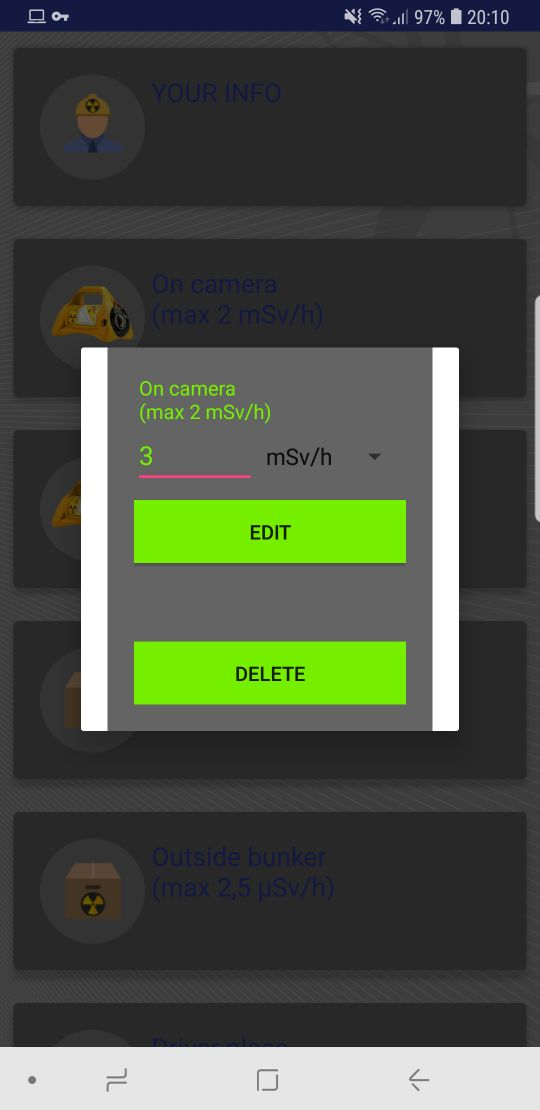
\includegraphics[scale=0.2]{img/soft/onCamera3MSV.jpeg}
       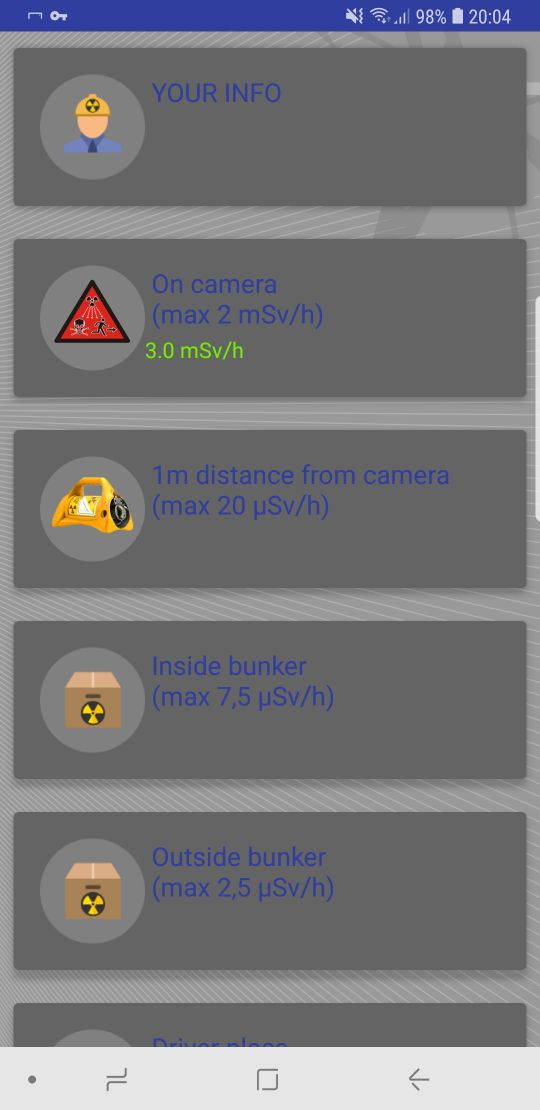
\includegraphics[scale=0.2]{img/soft/safetyAlarmForCamera.jpeg}
        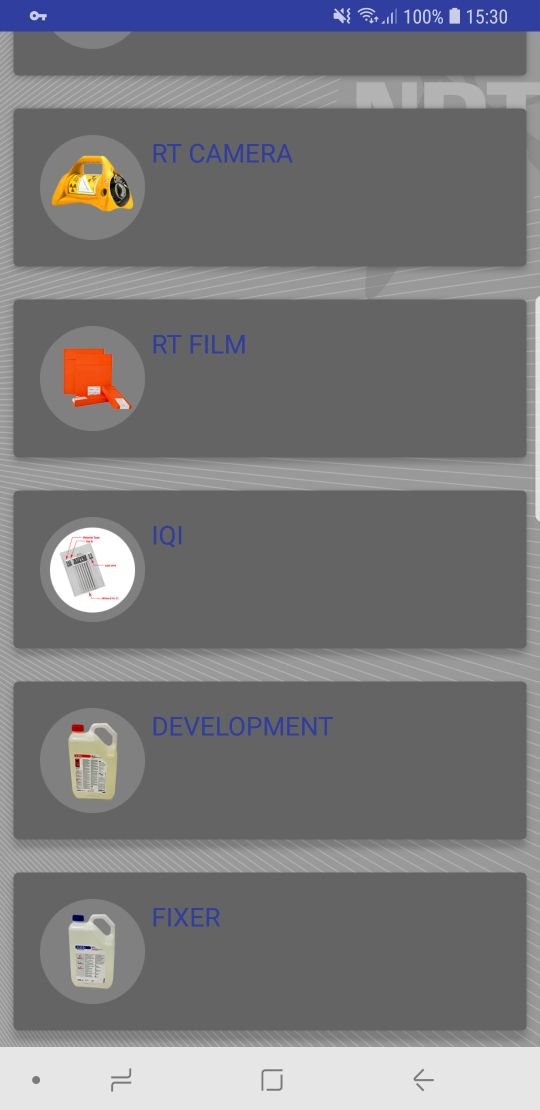
\includegraphics[scale=0.2]{img/soft/materials.jpeg}
         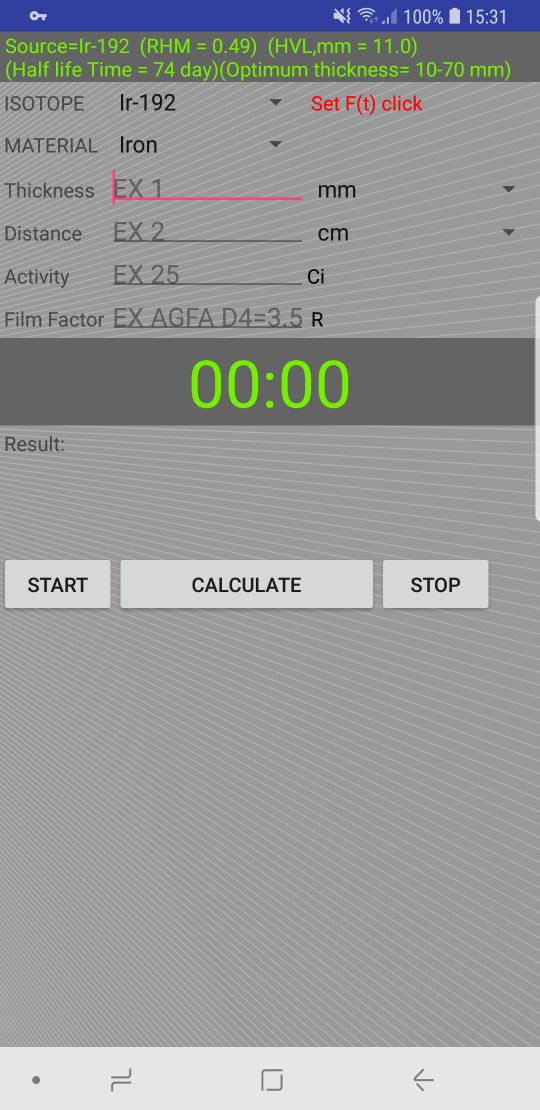
\includegraphics[scale=0.2]{img/soft/time.jpeg}\\
         
         
  \caption{Android-Client Radiographer}
  \label{sec:rg}
\end{figure}

\begin{figure}[htb]

            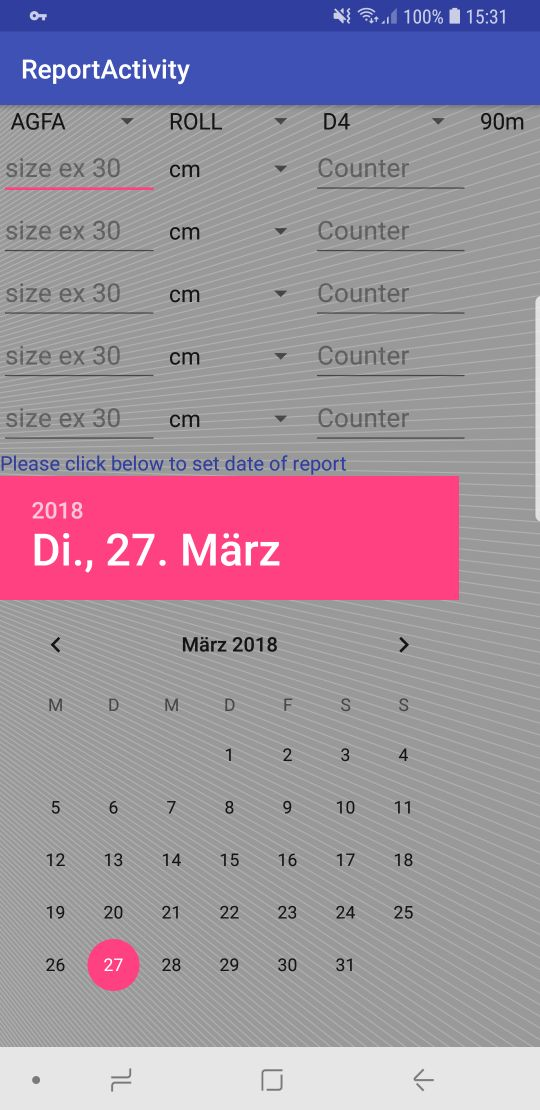
\includegraphics[scale=0.2]{img/soft/report.jpeg}
       		 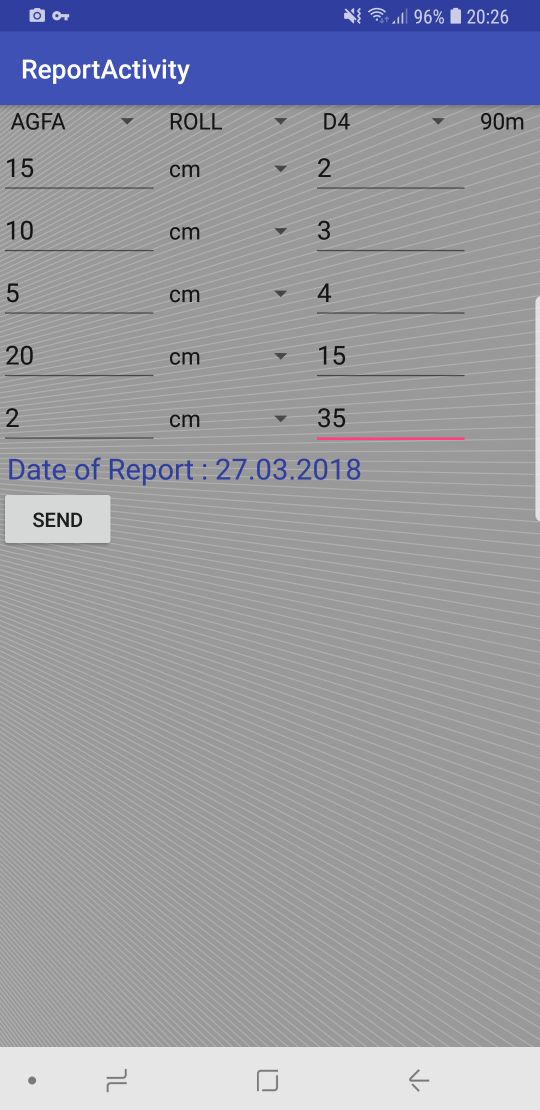
\includegraphics[scale=0.2]{img/soft/reportDate.jpeg}
              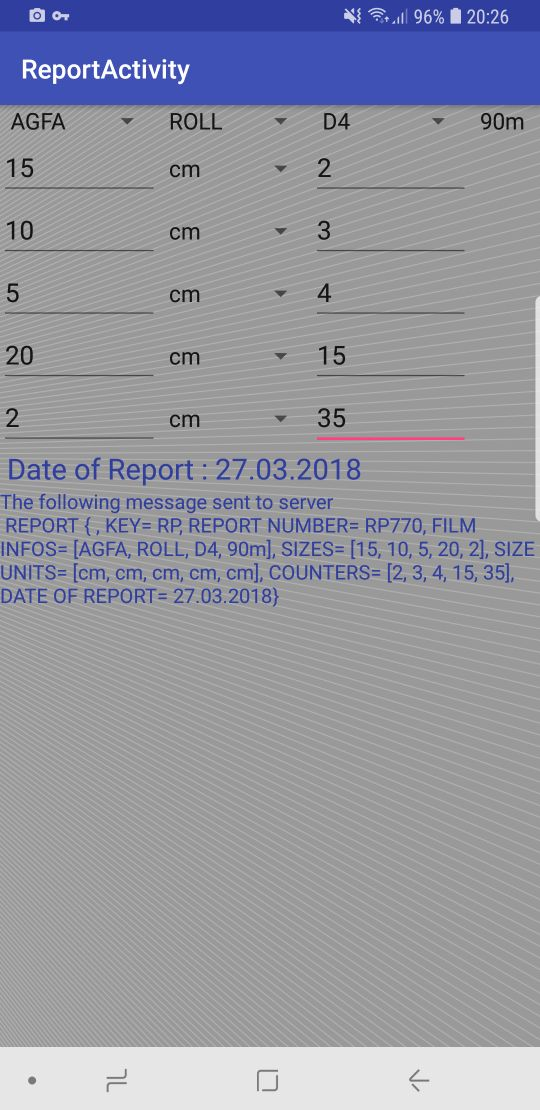
\includegraphics[scale=0.2]{img/soft/sendReport.jpeg}
               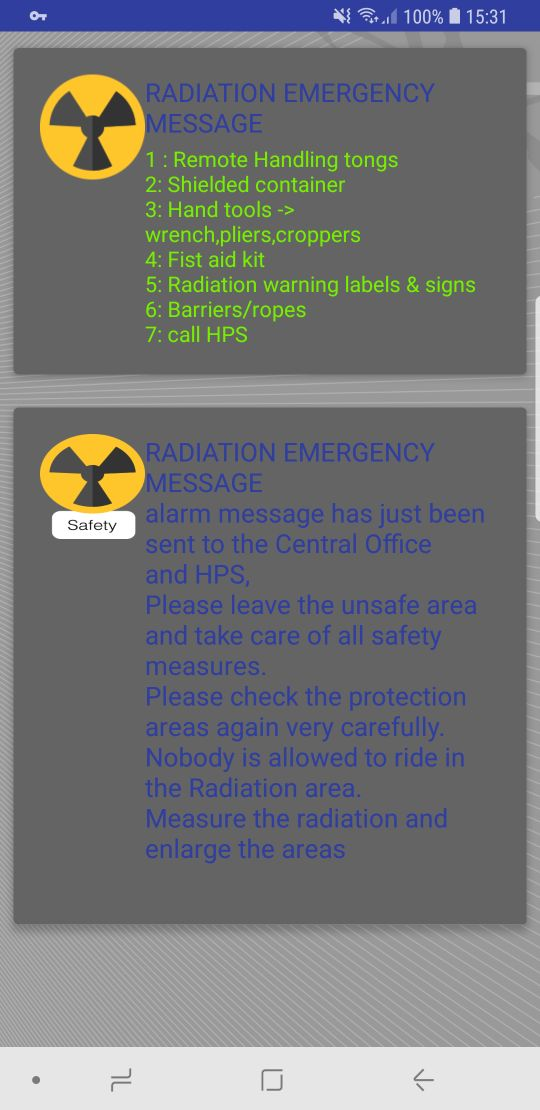
\includegraphics[scale=0.2]{img/soft/alarm.jpeg}\\
\caption{Android-Client Radiographer}
  \label{sec:rg2} 
\end{figure}
%=====================UML=================================
\chapter{UML Graphen}
\subsection{Model}

\begin{figure}
\centering
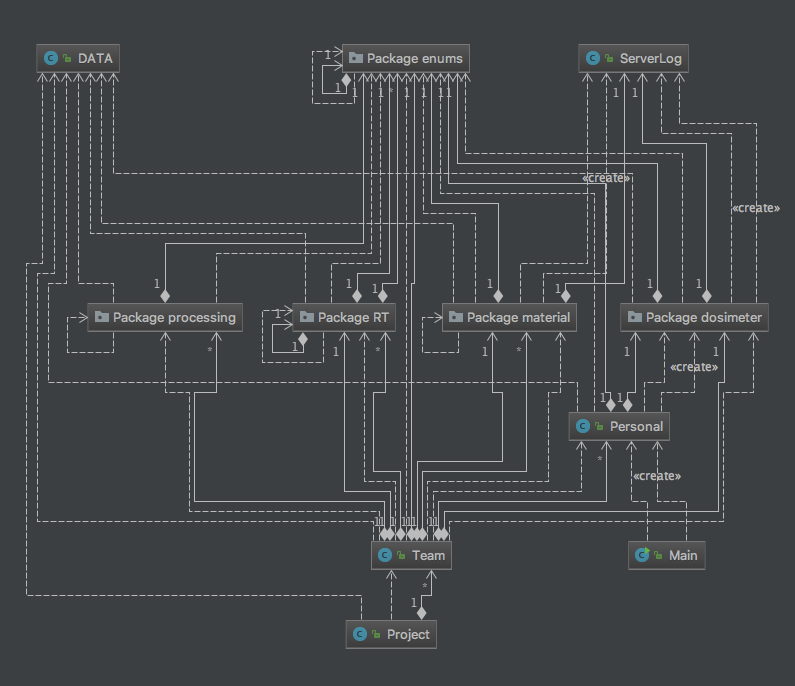
\includegraphics[scale=0.6]{img/diagrams/modelDiagram.png}
 \caption{Model}
 \label{sec:model}
\end{figure}

\begin{figure}
\centering
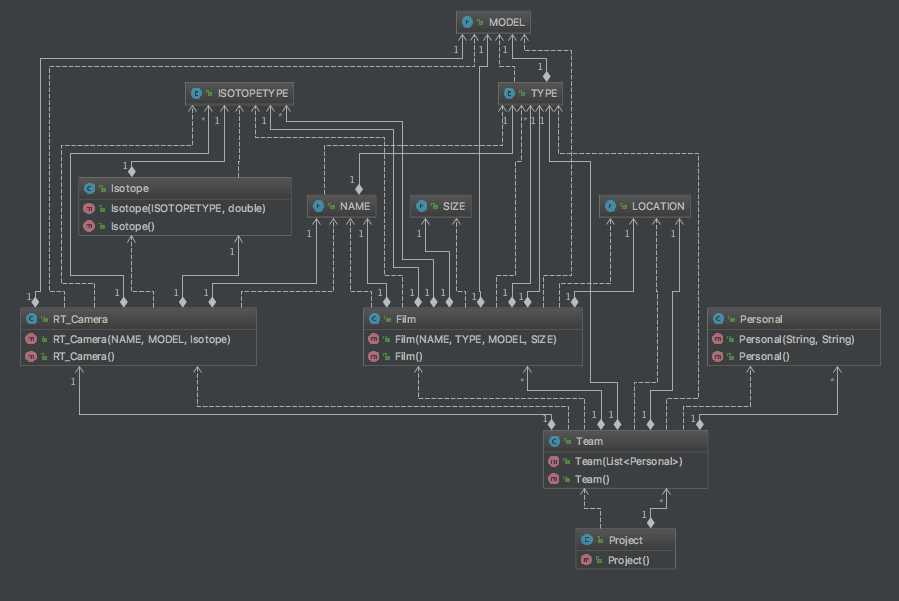
\includegraphics[scale=0.6]{img/diagrams/software.png}
 \caption{Server Model}
 \label{sec:servermodel}
\end{figure}



\begin{figure}
\centering
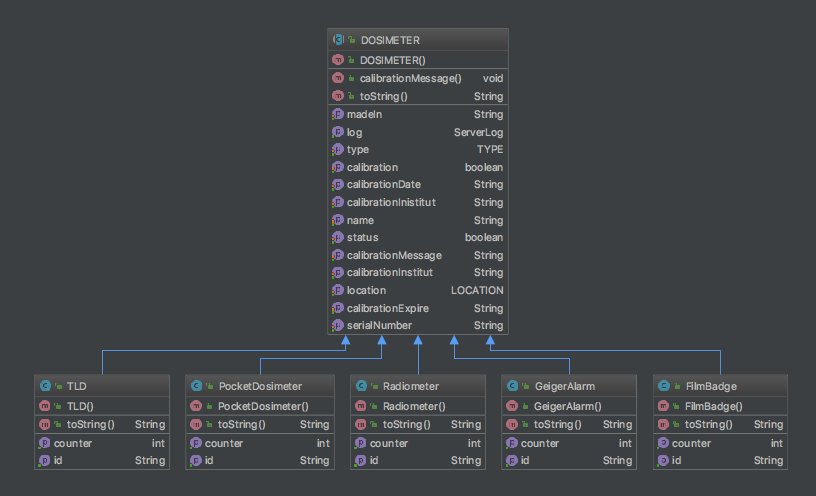
\includegraphics[scale=0.6]{img/diagrams/dosimeter.png}
 \caption{dosimeter}
 \label{sec:Dosimeter}
\end{figure}

\begin{figure}
\centering
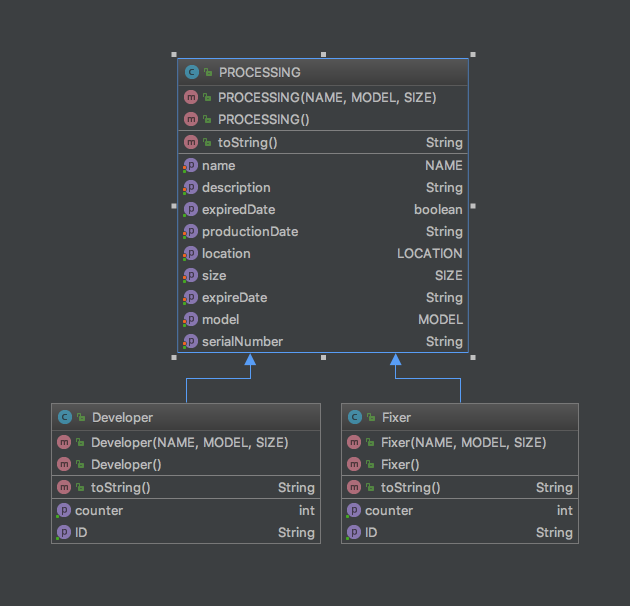
\includegraphics[scale=0.6]{img/diagrams/processing.png}
 \caption{Processing}
 \label{sec:processing}
\end{figure}

\begin{figure}
\centering
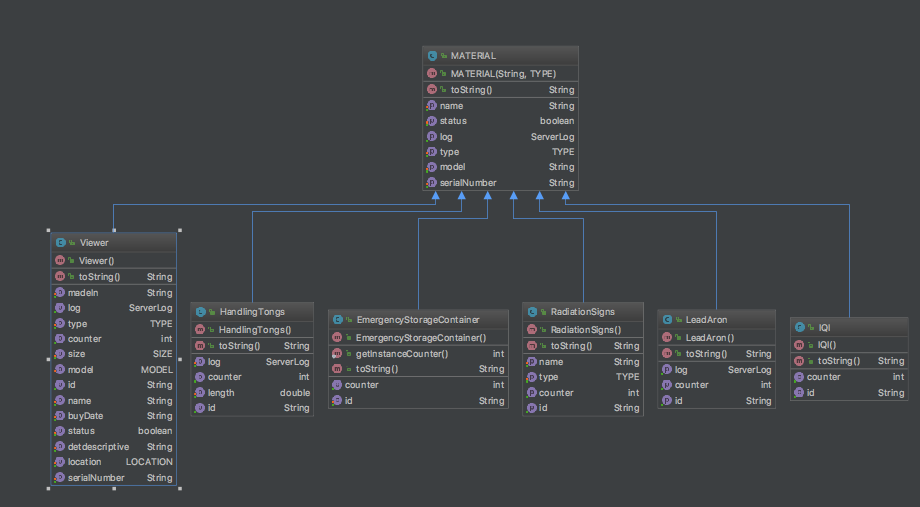
\includegraphics[scale=0.6]{img/diagrams/materials.png}
 \caption{Materials}
 \label{sec:materials}
\end{figure}









































